% !TEX TS-program = pdflatex
% !TEX encoding = UTF-8 Unicode

% This file is a template using the "beamer" package to create slides for a talk or presentation
% - Giving a talk on some subject.
% - The talk is between 15min and 45min long.
% - Style is ornate.

% MODIFIED by Jonathan Kew, 2008-07-06
% The header comments and encoding in this file were modified for inclusion with TeXworks.
% The content is otherwise unchanged from the original distributed with the beamer package.

\documentclass{beamer}

\mode<presentation>
{
  \usetheme{Malmoe}
  % or ...

  %\setbeamercovered{transparent}
  % or whatever (possibly just delete it)
}


\usepackage{tikz}
\usetikzlibrary{arrows,shapes,positioning}
\usepackage[english]{babel}
\usepackage{graphicx}
\usepackage{amssymb}
\usepackage{multicol,multirow,array}
\setbeamertemplate{navigation symbols}{}%remove navigation symbols
\setbeamertemplate{footline}
{
  \leavevmode%
  \hbox{%
  \begin{beamercolorbox}[wd=.4\paperwidth,ht=2.25ex,dp=1ex,center]{author in head/foot}%
    \usebeamerfont{author in head/foot}\insertshortauthor
  \end{beamercolorbox}%
  \begin{beamercolorbox}[wd=.6\paperwidth,ht=2.25ex,dp=1ex,center]{title in head/foot}%
    \usebeamerfont{title in head/foot}\insertshorttitle\hspace*{3em}
    \insertframenumber{} / \inserttotalframenumber\hspace*{1ex}
  \end{beamercolorbox}}%
  \vskip0pt%
}
\makeatletter
%\setbeamertemplate{footline}[frame number]
\setbeamertemplate{headline}{}

\title[X Chromosome Association Testing in HCHS/SOL] % (optional, use only with long paper titles)
{X Chromosome Association Testing in HCHS/SOL}

%\subtitle
%{Presentation Subtitle} % (optional)

\author[Caitlin McHugh, with Tim Thornton] % (optional, use only with lots of authors)
{Caitlin McHugh, with Tim Thornton}
% - Use the \inst{?} command only if the authors have different
%   affiliation.

\institute[University of Washington] % (optional, but mostly needed)
{
  Department of Biostatistics\\
  University of Washington
}
% - Use the \inst command only if there are several affiliations.
% - Keep it simple, no one is interested in your street address.

\date[Short Occasion] % (optional)
{27 March 2015}

% If you have a file called "university-logo-filename.xxx", where xxx
% is a graphic format that can be processed by latex or pdflatex,
% resp., then you can add a logo as follows:

% \pgfdeclareimage[height=0.5cm]{university-logo}{university-logo-filename}
% \logo{\pgfuseimage{university-logo}}

% If you wish to uncover everything in a step-wise fashion, uncomment
% the following command: 

%\beamerdefaultoverlayspecification{<+->}


\begin{document}

\begin{frame}
  \titlepage
\end{frame}

\begin{frame}{Outline}
\tableofcontents
 % You might wish to add the option [pausesections]
\end{frame}

\section{MLM-X: Mixed Model Association on the X Chromosome}
\begin{frame}{Mixed Model Association Mapping}
\begin{itemize}
\item For association testing with an \textit{autosomal} SNP, the following model has been proposed
\begin{equation} Y = \beta_0 + \beta_1 \mbox{SNP} + g_A + \mbox{covariates} +\epsilon
\end{equation} where
$$ g_A \sim MVN(0,\sigma_A^2 \mathbf{\Phi_A})$$
$$ \epsilon \sim MVN(0,\sigma_\epsilon^2 \mathbb{I})$$
\item For detecting association on the X chromosome, we propose the following \textcolor{blue}{MLM-X} model
\begin{equation}
 Y = \beta_0 + \beta_1 \mbox{SNP}_X + g_A + g_X + \mbox{covariates} +\epsilon
\end{equation} with an additional random component for polygenic effects on the X chromosome
$$ g_X \sim MVN(0,\sigma_X^2 \mathbf{\Phi_X})$$
\end{itemize}
% g_x and g_a are terms to adjust for background polygenic effects due to the autosomes and x chr
% we want to fit these terms separately since we've proven genetics on the autosome and x chr are different
\end{frame}

\begin{frame}{Sample Structure}
\begin{itemize}
\item GWAS often have sample structure, including population stratification, family structure and/or cryptic relatedness.
\item It is well known that failure to appropriately account for sample structure can lead to spurious association and reduced power.
\item SNP data can be used to infer recent relatedness (family structure) and more distant relatedness (population structure).
\end{itemize}
\end{frame}

%
%\begin{frame}{Association Testing Model, in a Graph}
%\begin{center} 
%\begin{tikzpicture}
%[place/.style={rectangle,draw=white!10,fill=white!20,thick},
%transition/.style={rectangle,draw=white!50,fill=white!20,thick}]
%%\node[place] (ancestry) {Ancestry};
%\node[transition](placeholder) {};
%\node[place](genotype) [left=of placeholder]{Genotype};
%%edge [<-](ancestry);
%\node[place](trait) [right=of placeholder]{Phenotype}
%edge[<-](genotype);
%%edge[<-](ancestry);
%\end{tikzpicture}
%\end{center}
%\end{frame}
%
%\begin{frame}{Association Testing Model, in a Graph}
%\begin{center} 
%\begin{tikzpicture}
%[place/.style={rectangle,draw=white!10,fill=white!20,thick},
%transition/.style={rectangle,draw=white!50,fill=white!20,thick}]
%\node[place] (ancestry) {Ancestry};
%\node[transition](placeholder) [below=of ancestry]{};
%\node[place](genotype) [left=of placeholder]{Genotype}
%edge [<-](ancestry);
%\node[place](trait) [right=of placeholder]{Phenotype}
%edge[<-](genotype)
%edge[<-](ancestry);
%\end{tikzpicture}
%\end{center}
%\end{frame}
%
%\begin{frame}{How Does the X Chromosome Factor In?}
%Should we adjust for autosomal relatedness and structure \textit{and} X chromosome relatedness and structure?\\
% \vspace{1cm}
%\begin{center} 
%\begin{tikzpicture}
%[place/.style={rectangle,draw=white!10,fill=white!20,thick},
%transition/.style={rectangle,draw=white!50,fill=white!20,thick}]
%\node[place] (ancestry) {Ancestry};
%\node[transition](placeholder) [below=of ancestry]{};
%\node[place](xchr) [right=of placeholder]{X Chr}
%edge [<-](ancestry);
%\node[place](trait) [below=of xchr]{Phenotype}
%edge[<-](xchr);
%\node[place](autosomal) [left=of placeholder]{Autosomal}
%edge[<-](ancestry)
%edge[->](trait);
%\node[place](genotype) [below=of autosomal]{X Chr Genotype}
%edge[->](trait)
%edge[<-](xchr);
%\draw[->](autosomal) to node [auto,swap]{?} (genotype);
%\end{tikzpicture}
%\end{center}
%\end{frame}


\section{Estimating Family Structure on the X Chromosome}
\begin{frame}{Genetic Relatedness on the X Chromosome: $\mathbf{\Phi_X}$}
\begin{itemize}
%\item We will call the X chromosome kinship matrix `$\mathbf{\Phi_X}$.'
\item The X chromosome kinship coefficient between individuals $i$ and $j$, $\Phi^X_{ij}$,  is defined as the probability of sampling one allele IBD at random from individual $i$ and individual $j$ on the X chromosome.
\item \textit{Note} for males there is no randomness in sampling, as there is only one allele at each location on the X chromosome.
\end{itemize}
\end{frame}

\begin{frame}
\begin{columns}
    \begin{column}{0.3\textwidth}
      \centering
      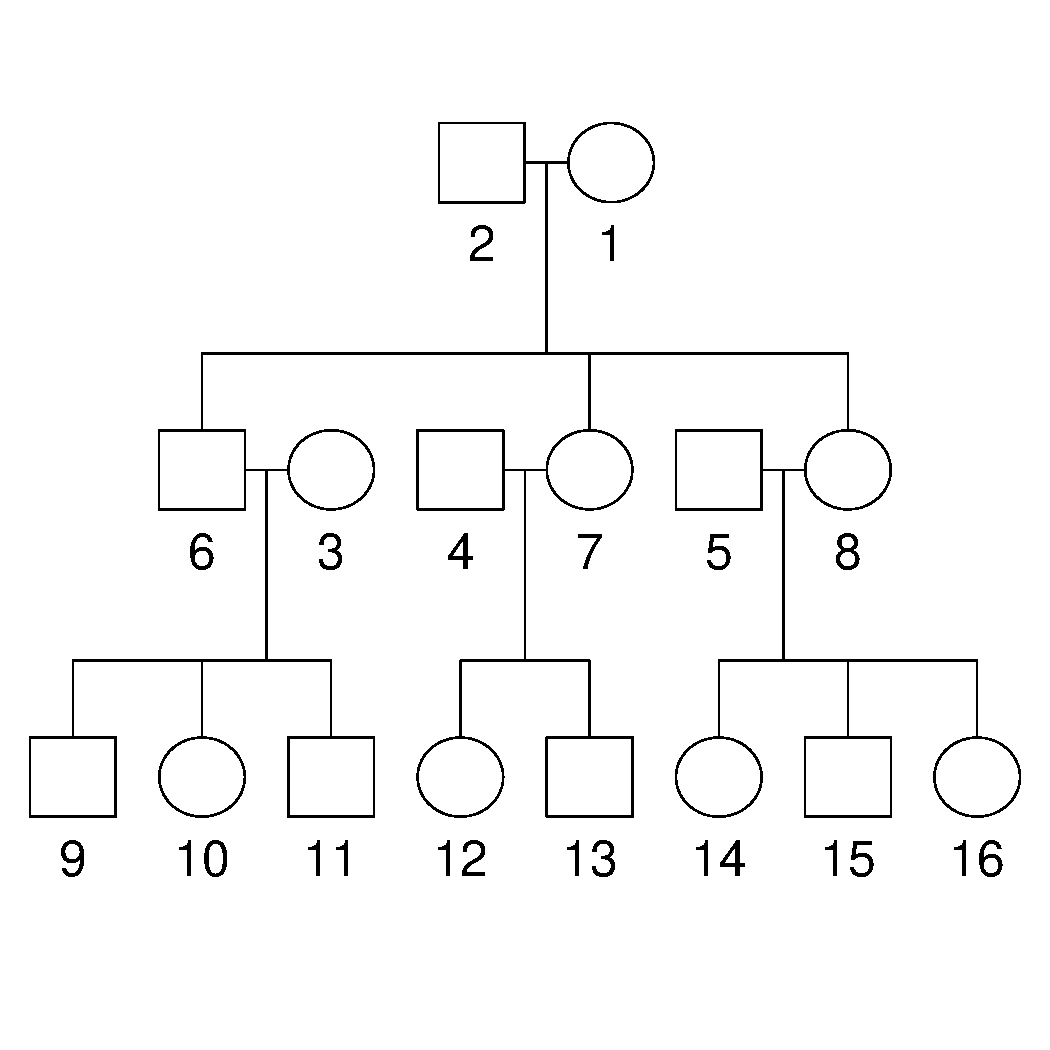
\includegraphics[height=4.5cm]{../pedigree_16individs.pdf}
    \end{column}
    \begin{column}{0.5\textwidth}
      \centering
      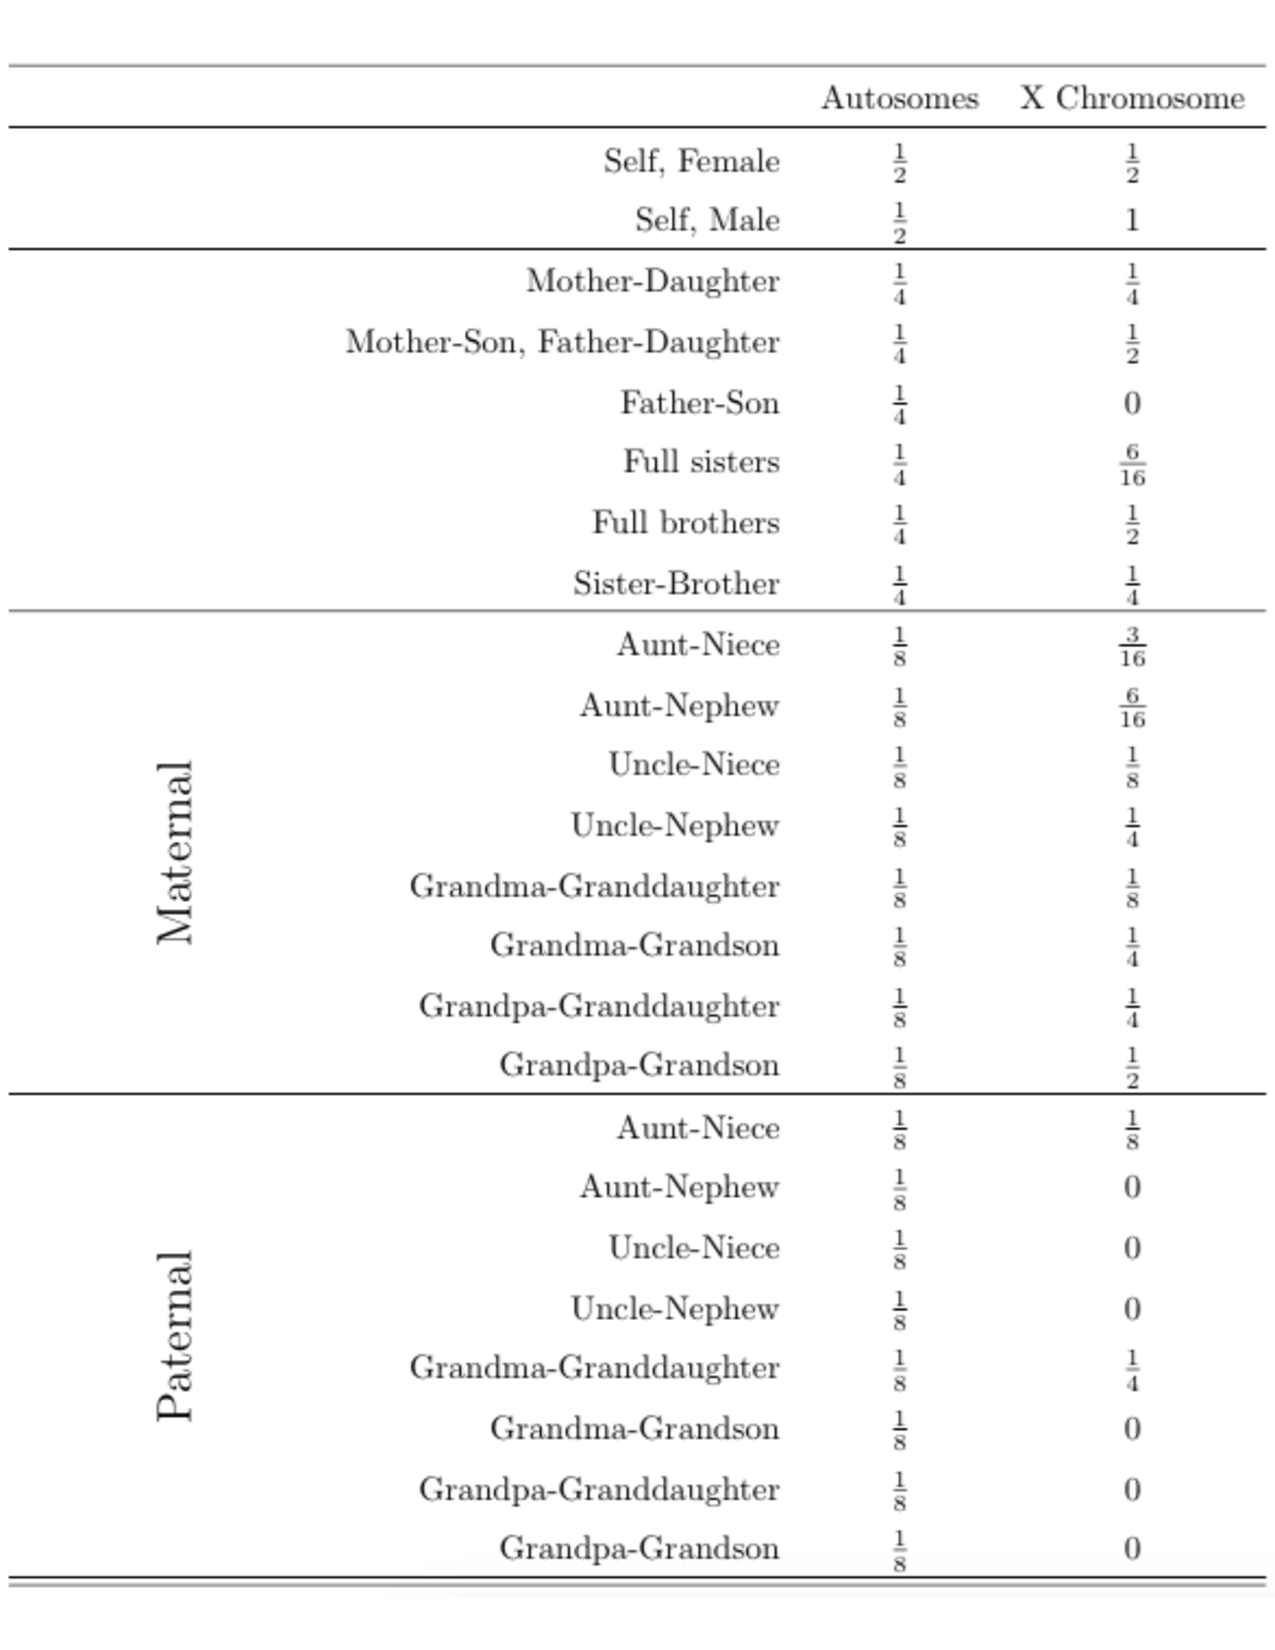
\includegraphics[height=8.3cm]{../olga_presentation_26jan15/xchr_kc_values.pdf}
    \end{column}
 \end{columns}
\end{frame}

\begin{frame}{Estimating $\mathbf{\Phi_X}$}
\begin{itemize}
%\item We assume a total of $N$ X chromosome SNPs; males coded 0, 2 and females coded 0, 1, 2.
\item We can estimate $\mathbf{\Phi_X}$ using the following GRM equations:
\begin{align*}
\mbox{GR}_{FF}&=\frac{1}{N}\frac{\sum_{i=1}^N (X_{iF}-2p_i)(X_{iF}-2p_i)}{\sum_{i=1}^N 2p_i(1-p_i)}\\
\mbox{GR}_{MM}&=\frac{1}{N} \frac{\sum_{i=1}^N(X_{iM}-p_i)(X_{iM}-p_i)}{\sum_{i=1}^Np_i(1-p_i)}\\
\mbox{GR}_{MF}&=\frac{1}{N}\frac{\sum_{i=1}^N (X_{iM}-p_i)(X_{iF}-2p_i)}{\sum_{i=1}^N \sqrt{2}p_i(1-p_i)}
\end{align*}
\end{itemize}where $F$ indicates a female and $M$ is a male.
\end{frame}

\begin{frame}{HCHS/SOL Samples, For Example}
\begin{figure}
\centering
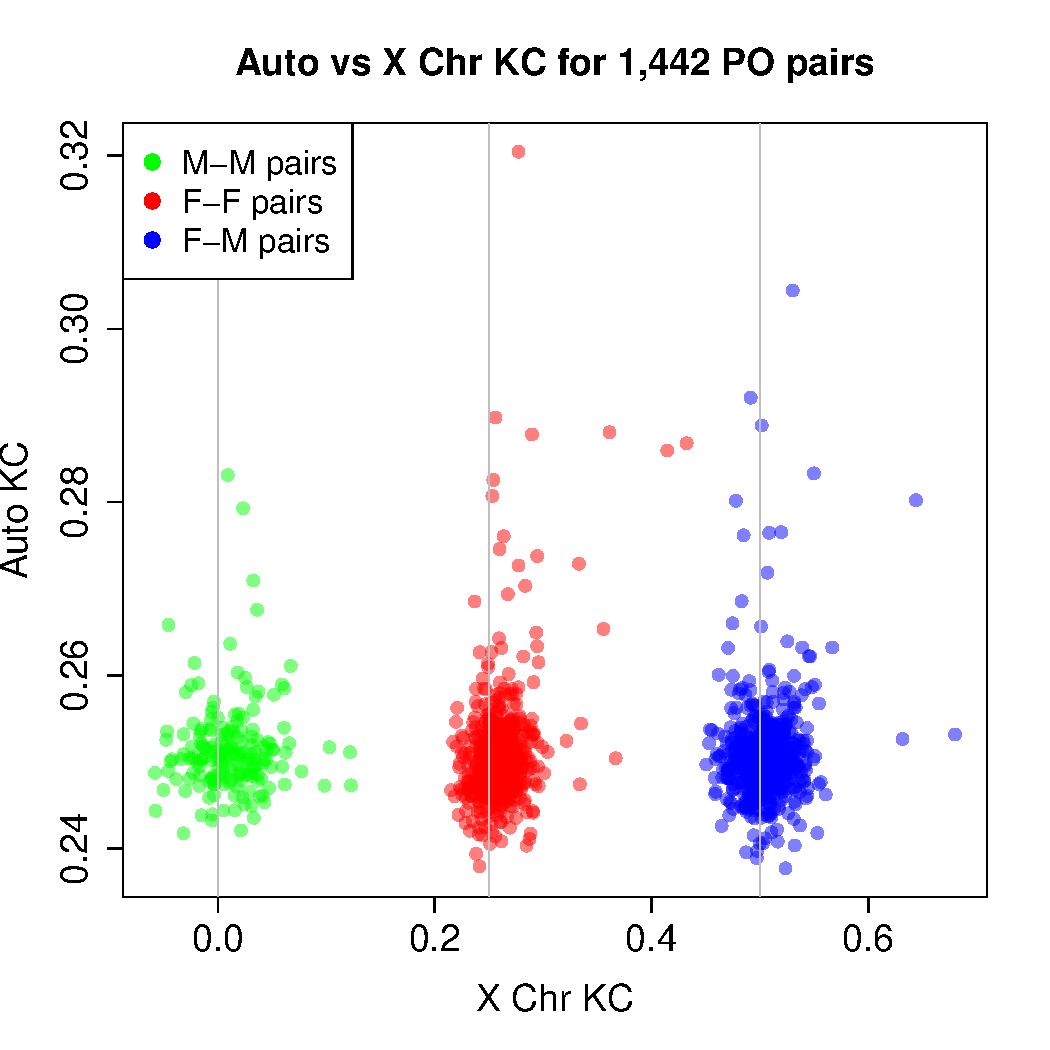
\includegraphics[height=7.8cm]{../kc_xPrunedvsAuto_poPairs_xAdj.pdf}
\end{figure}
\end{frame}


\section{Inferring Population Structure on the X Chromosome}
\begin{frame}{Population Structure on the X Chromosome}
We performed PCA using 3,600 LD pruned X chromosome SNPs.
\begin{figure}
\centering
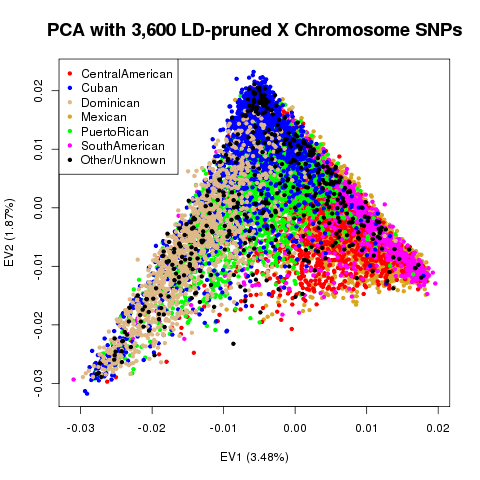
\includegraphics[height=6.3cm]{../pca_x_ev12_col.png}
\end{figure}
Can we control for this structure by simply adjusting for the autosomal PCs?
\end{frame}

\begin{frame}{Population Structure on the X Chromosome}
\begin{figure}
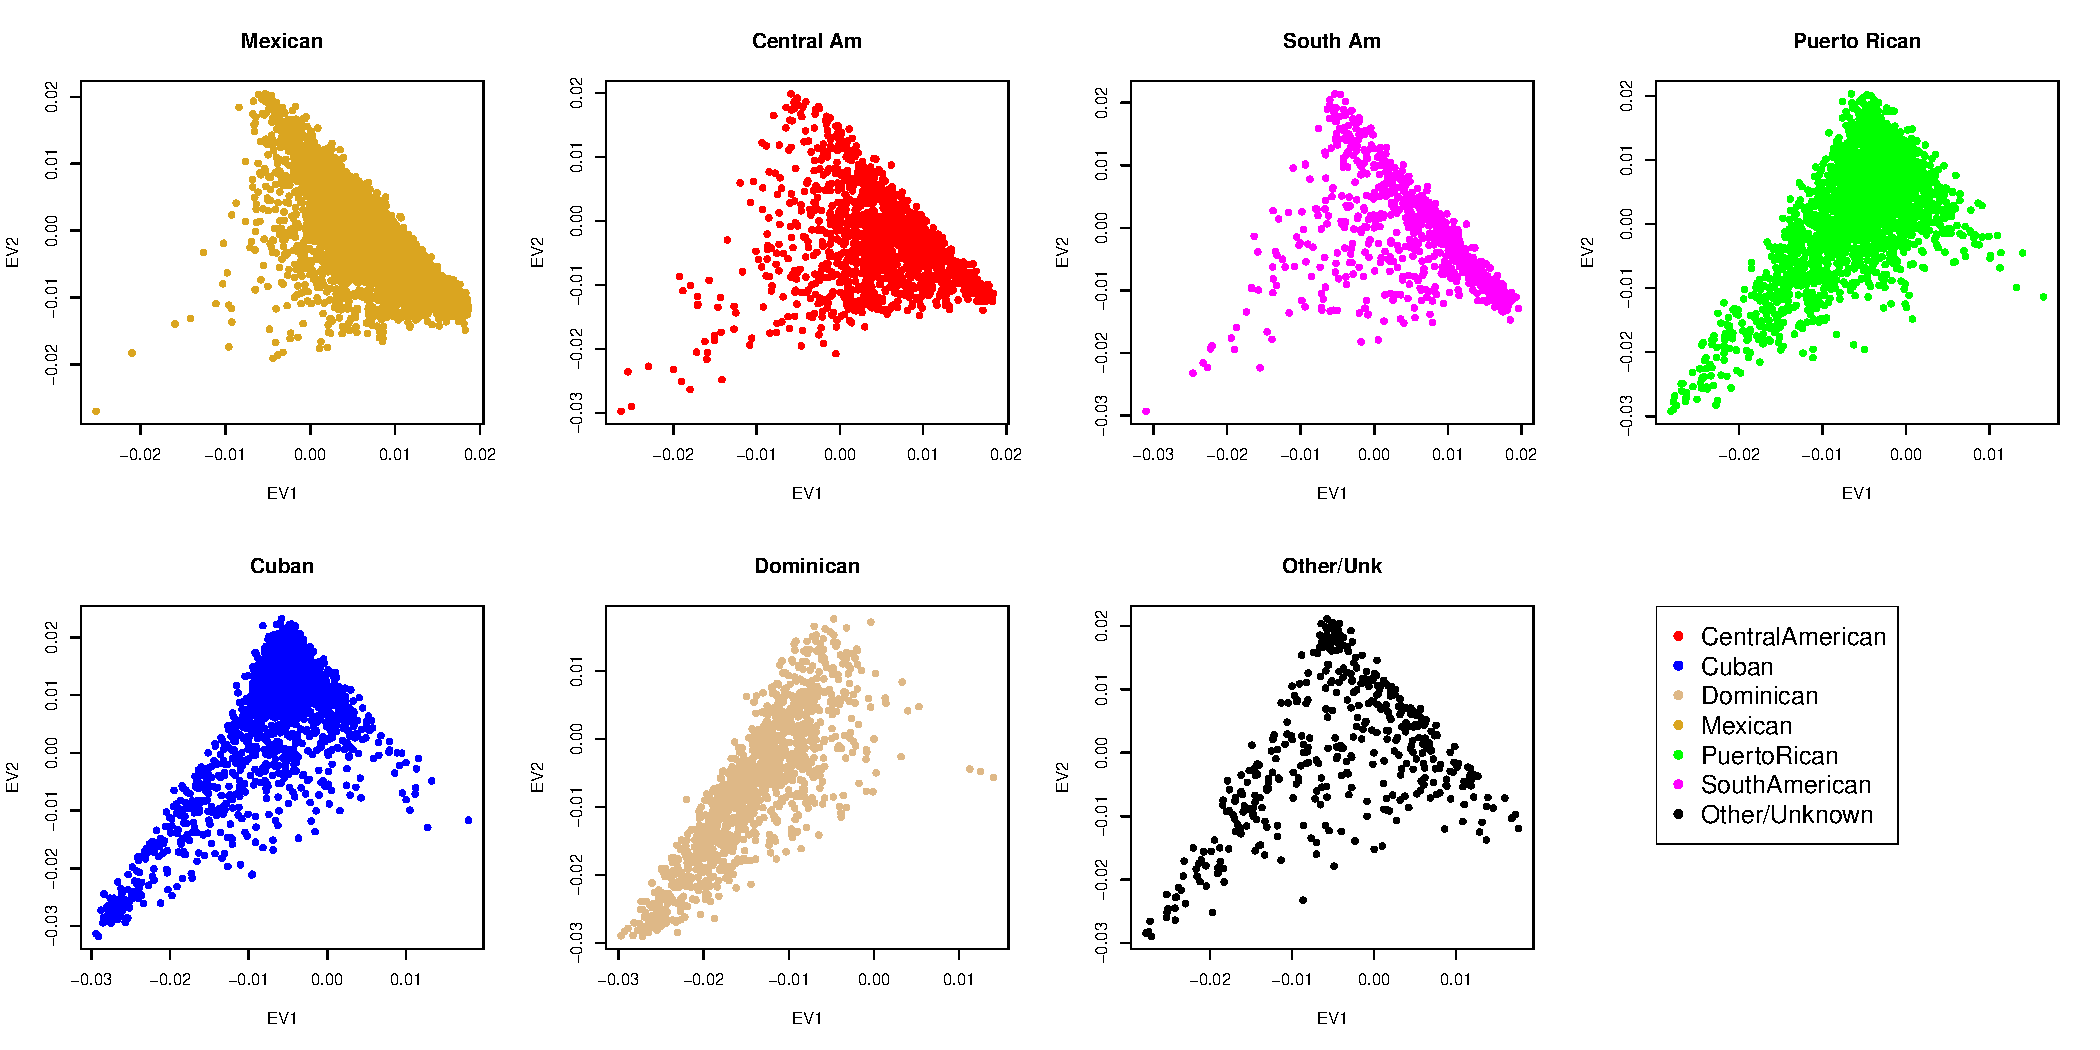
\includegraphics[height=6cm]{../pca_x_ev12_eachCol.pdf}
\end{figure}
\end{frame}

\begin{frame}{Population Structure on the X Chromosome, Beyond the Autosomes}
We estimated PCs on the X chromosome after adjusting for autosomal PCs 1-5.\\ 
\begin{figure}
\centering
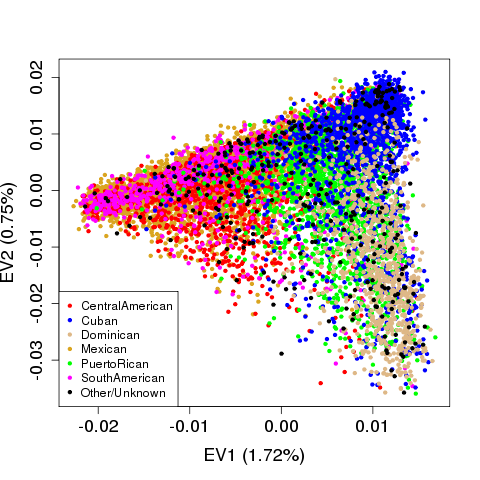
\includegraphics[height=6cm]{../eigen_unrel_adjXkc_adjAutoPC15_xPrunedKC_ev12_col.png}
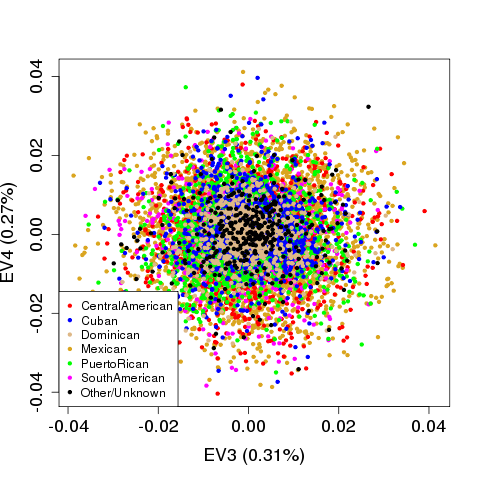
\includegraphics[height=6cm]{../eigen_unrel_adjXkc_adjAutoPC15_xPrunedKC_ev34_col.png}
\end{figure}
\end{frame}

\begin{frame}{Population Structure on the X Chromosome?}
We estimated PCs on the X chromosome after adjusting for X chromosome PCs 1-2.
\begin{figure}
\centering
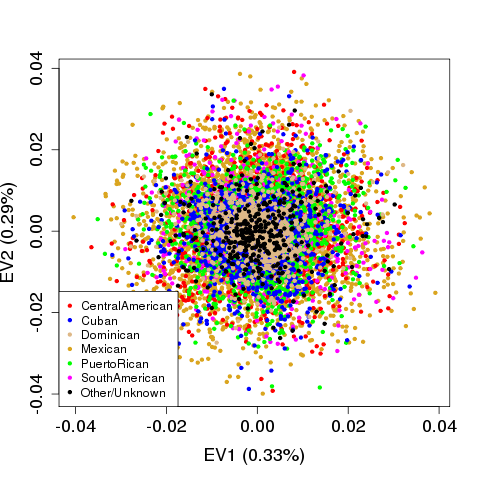
\includegraphics[height=7.3cm]{../eigen_unrel_adjxPrunedKC_adjxPC12_ev12_col.png}
\end{figure}
\end{frame}


\begin{frame}{Global Ancestry Across the Genome}
\begin{figure}
\centering
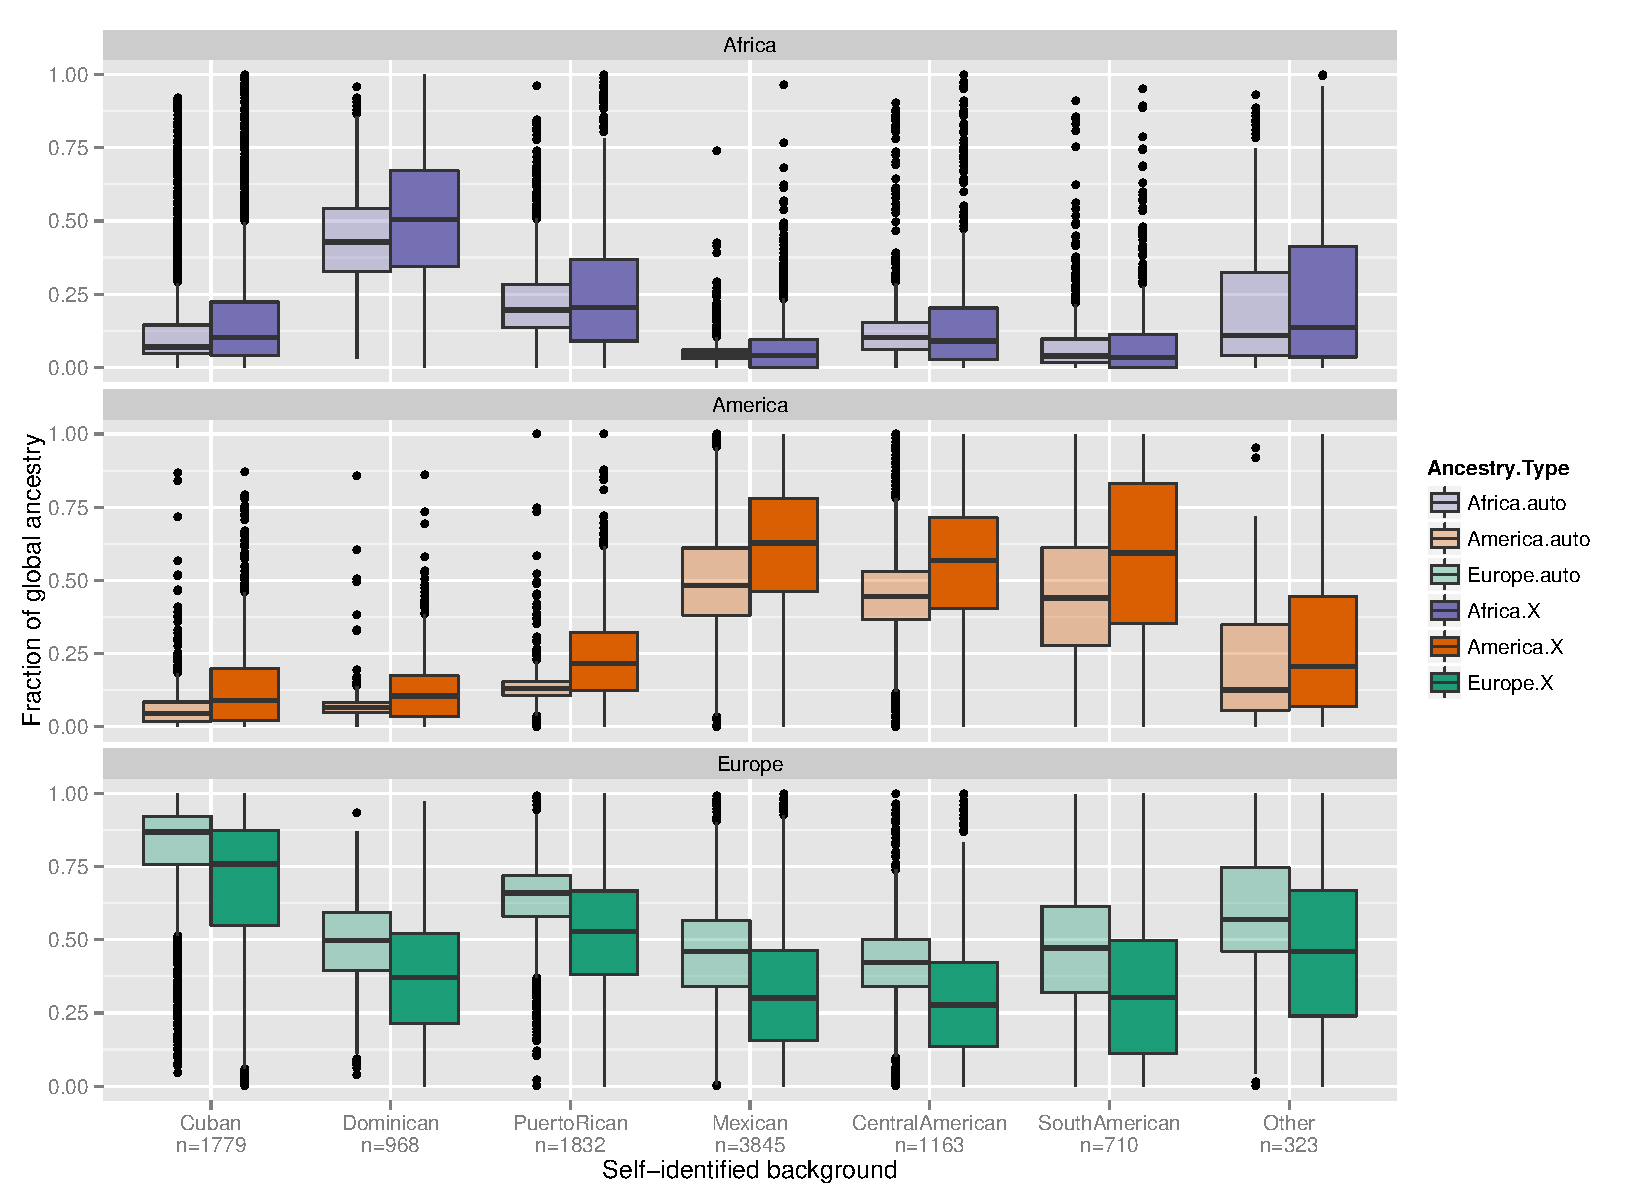
\includegraphics[height=7.8cm]{../admixture_xchrAutoComp_k3_boxplots.pdf}
\end{figure}
\end{frame}

\begin{frame}{Global Ancestry Difference Between X Chr \& Autosomes}
\begin{figure}
\centering
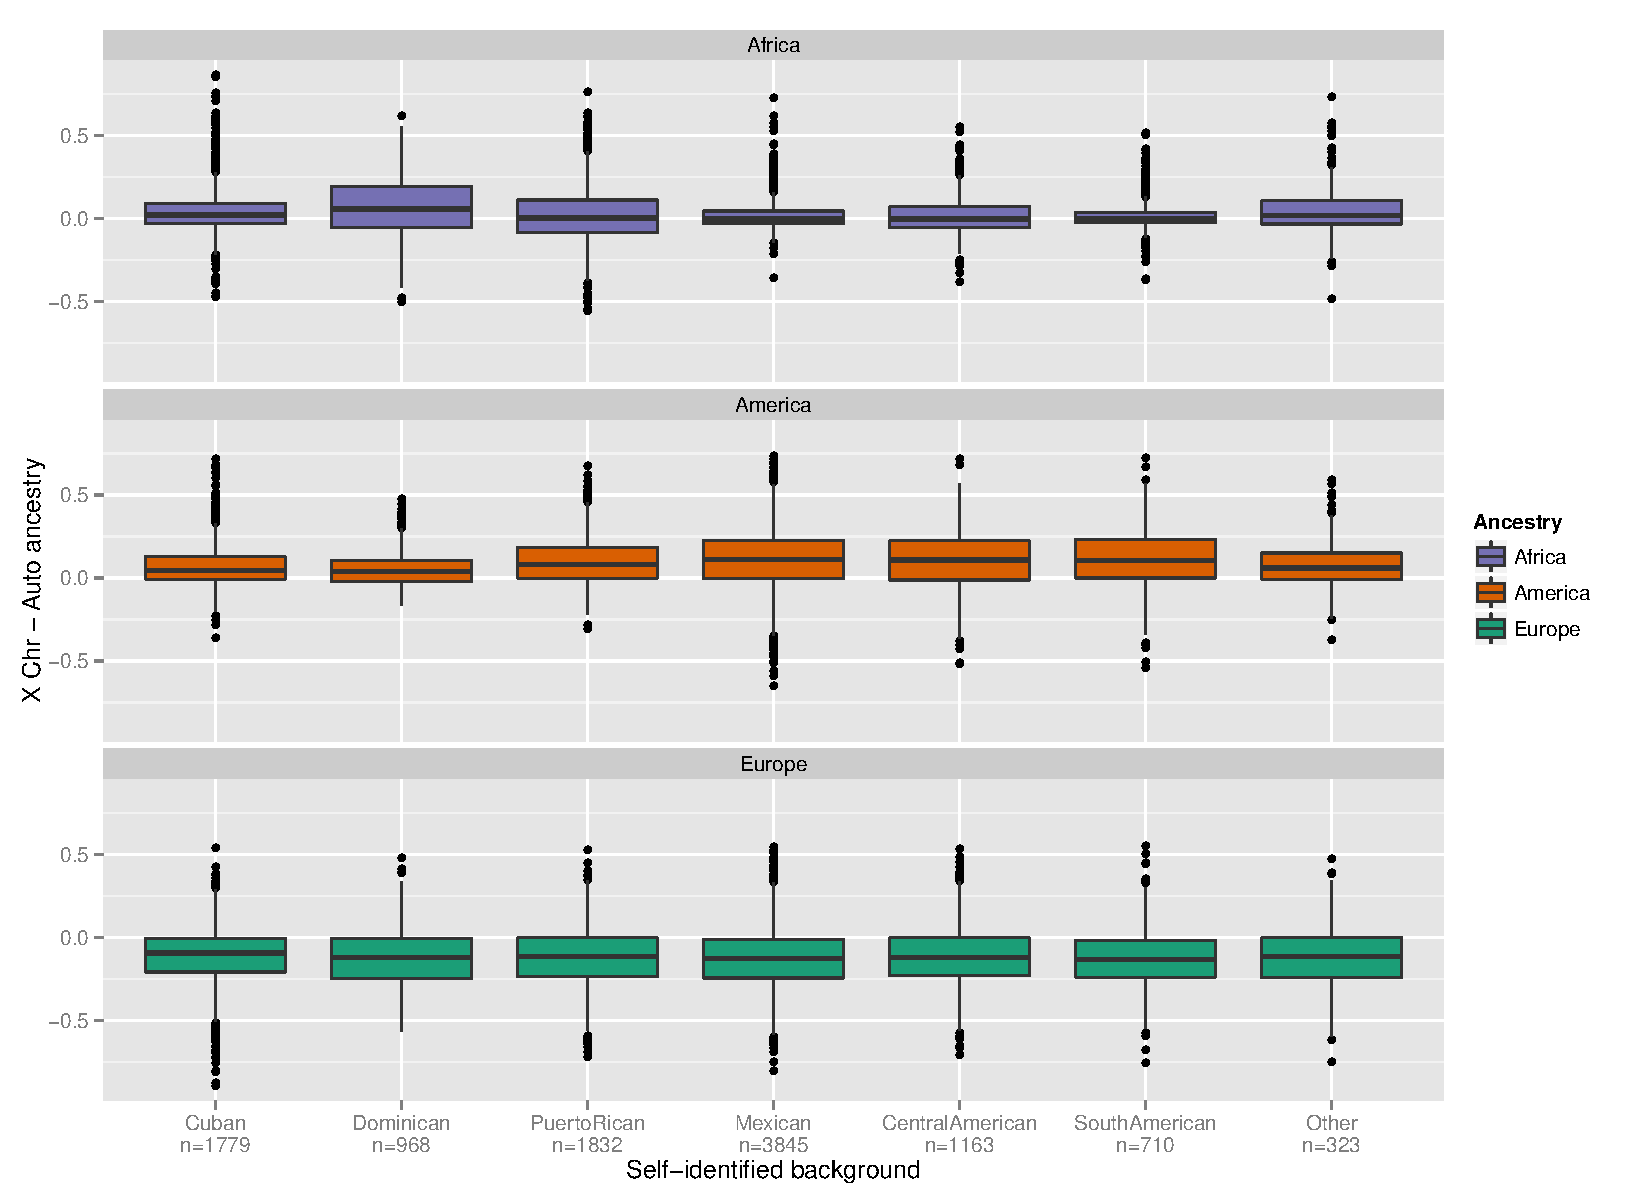
\includegraphics[height=7.8cm]{../admixture_xchrAutoDiff_k3_boxplots.pdf}
\end{figure}
\end{frame}


\section{Application to RBC Trait}

\begin{frame}{Red Blood Cell Count}
\begin{itemize}
\item We performed a GWAS with the red blood cell count (RBC) trait. 
\item RBC was previously found to be associated with variants in gene G6PD on Xq28 in African Americans.
\item We found the Xq28 region to be associated with RBC in the HCHS/SOL samples, when applying the autosomal mixed model and the MLM-X model.
\end{itemize}
\end{frame}

\begin{frame}{`Autosomal Model'\footnote{these are as described in the working group previously}}
We include all individuals with non-missing outcome and covariates, exclude Asian outliers identified with PCA and additionally exclude samples with
\begin{itemize}
\item blood/lymph malignant tumor
\item bone cancer
\item pregnancy
\item chronic kidney disease
\item chemotherapy
\item \% blasts $>$5
\item \% immature granulocytes $>$5
\end{itemize}
Fixed effect covariates included are sex, age, center, and autosomal ancestry eigenvectors 1-5.\\
We include random effects of block group, household and autosomal kinship.
\end{frame}

\begin{frame}{Previous Variance Component Estimates, n=12,502}
\begin{table}[h!]
\centering
\begin{tabular}{ccc}
  \hline
& estimate & 95\% CI \\ \hline
block group & 0.00363 & (-0.00177, 0.00903)\\
household &0.04945 & (0.02113, 0.07777)\\
autosomal kinship &0.28473 &(0.23215, 0.33732)\\
environment & 0.66218& (0.60989, 0.71448) \\ \hline
\end{tabular}
\caption{Estimate (95\% CI) of the proportion variance for each of the components.}
\label{table:varComp}
\end{table}
\end{frame}

\begin{frame}{Previous Genome-Wide Assoc Test Results, n=12,502}
\centering
\begin{figure}
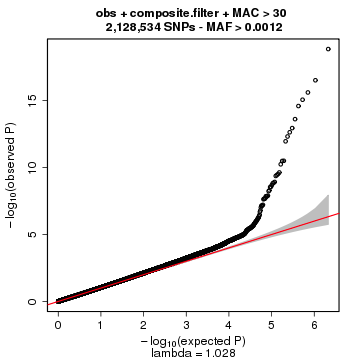
\includegraphics[height=4.6cm]{../RBC_MLM-X_results/qq_obs_rbc.png}\\
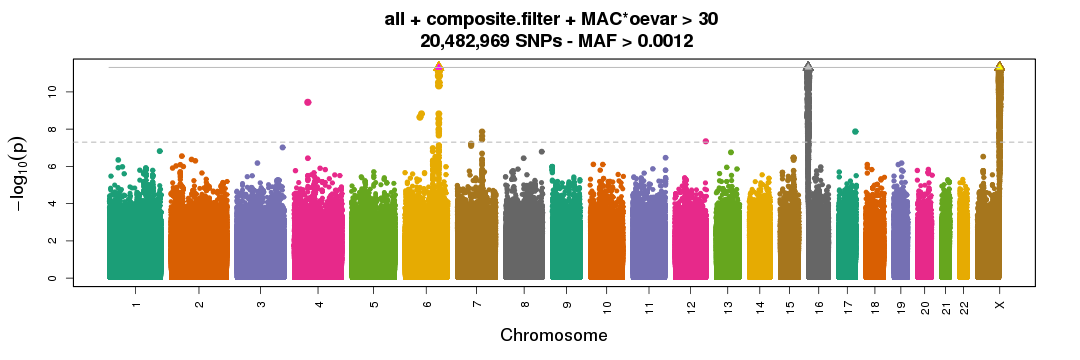
\includegraphics[width=11cm]{../RBC_MLM-X_results/pval_manh_single_2014-08-12_04-43-43_316987.png}
\end{figure}
\end{frame}

\begin{frame}{Previous X Chr Assoc Test Results, n=12,502}
\centering
\begin{figure}
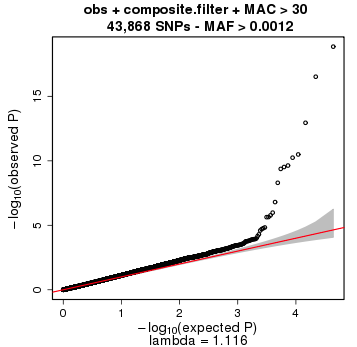
\includegraphics[height=4.6cm]{../RBC_MLM-X_results/pval_qq_filtered_2015-02-27_11-37-52_auto_316987_v2.png}\\
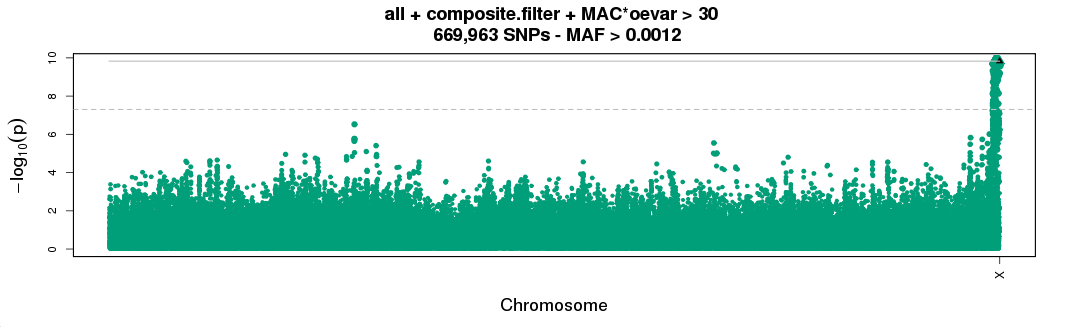
\includegraphics[width=11cm]{../RBC_MLM-X_results/pval_manh_single_2015-02-27_11-37-52_auto_316987_v2.png}
\end{figure}
\end{frame}

\begin{frame}{MLM-X Model}
We include all individuals with non-missing outcome and covariates, exclude Asian outliers identified with PCA and additionally exclude samples with
\begin{itemize}
\item blood/lymph malignant tumor
\item bone cancer
\item pregnancy
\item chronic kidney disease
\item chemotherapy
\item \% blasts $>$5
\item \% immature granulocytes $>$5
\item \textbf{\textcolor{red}{an X chromosome anomaly}}
\end{itemize}
Fixed effect covariates included are sex, age, center, autosomal ancestry eigenvectors 1-5, and \textbf{\textcolor{red}{X chromosome ancestry eigenvectors 1-2}}.\\
We include random effects of block group, household, autosomal kinship and \textbf{\textcolor{red}{X chromosome kinship}}.
\end{frame}

\begin{frame}{MLM-X Variance Component Estimates, n=12,488}
\small
\begin{table}[h!]
\centering
\begin{tabular}{r|l||l}
  \hline
&MLM-X &Autosomal \\ \hline
%& estimate  (95\% CI)  & estimate (95\% CI) \\ \hline
block group & 0.00396 (-0.0016, 0.0095) & 0.00363 (-0.0018, 0.0090)\\
household &0.04950 (0.0209, 0.0781)& 0.04945  (0.0211, 0.0778)\\
autosomal kinship &0.28453 (0.2316, 0.3375) & 0.28473 (0.2322, 0.3373)\\
X kinship &0.02935 (0.0137, 0.0450) & \\
environment &0.63266 (0.5783, 0.6870) &  0.66218 (0.6099, 0.7145) \\ \hline
\end{tabular}
\caption{Estimate (95\% CI) of the proportion variance for each of the components.}
\label{table:varComp}
\end{table}
\end{frame}

\begin{frame}{MLM-X Assoc Test Results, n=12,488}
\centering
\begin{figure}
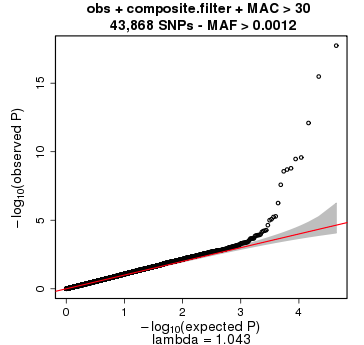
\includegraphics[height=4.6cm]{../RBC_MLM-X_results/pval_qq_filtered_2015-02-27_11-42-21___316987_v2.png}\\
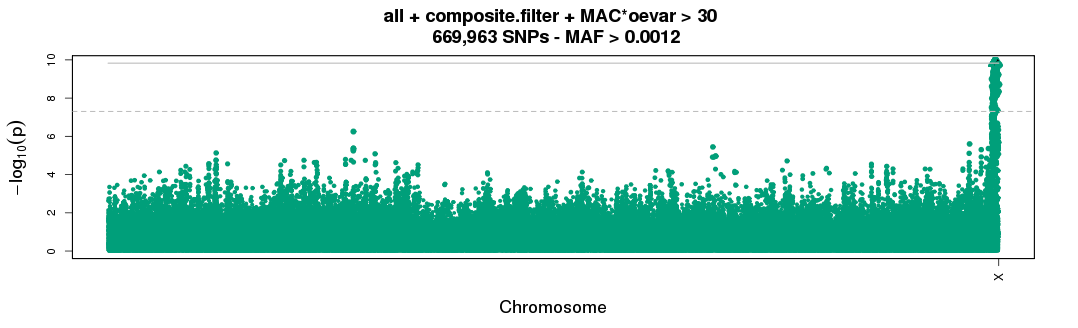
\includegraphics[width=11cm]{../RBC_MLM-X_results/pval_manh_single_2015-02-27_11-42-21___316987_v2.png}
\end{figure}
\end{frame}

\begin{frame}{Index SNP rs1050828}
\begin{table}[ht]
\centering
\begin{tabular}{r|lll}
  \hline
 & Effect Size (SE) & Stat & p-value \\ 
  \hline
autosomal & 0.1314 (0.0145) & 81.9377 & 1.40447e-19 \\ 
MLM-X & 0.1300 (0.0148) & 76.8729 & 1.82321e-18 \\ 
 \hline
\end{tabular}
\end{table}
\end{frame}

\end{document}


